\documentclass{article}
\usepackage[utf8]{inputenc}
\usepackage{graphicx}
\usepackage{hyperref}
\usepackage[utf8]{inputenc}
\usepackage{indentfirst}
\usepackage{amsmath,amssymb}


\DeclareMathOperator{\EX}{\mathbb{E}}% expected value

\title{BIOS 611 Project}
\author{Eric Zhang }
\date{}


\begin{document}

\maketitle
\tableofcontents

\newpage
\section{Introduction}
Bike sharing systems create an easy way for users to rent and return bikes through a network of kiosk locations. Especially in large cities, the use of bikes for transportation have become more abundant. Due to the nature of covariates involved in the decision making of renting a bike, this becomes an interesting problem for researchers to tackle. In this report, I uncover some relationships among the features and attempt to produce a model that is able to predict the number of bikes used given a feature vector.

\section{Data}
More information on the dataset can be found \href{https://www.kaggle.com/c/bike-sharing-demand/data}{here}.

\section{Preliminary Analysis}
First, we take a look at the covariates: season, holiday, workingday are categorical; weather, temp, atemp (temperature of what it feels like), humidity, windspeed are numerical. An obvious relationship might be the higher the temperature, the more bikes will be used because it's more enjoyable to bike in warmer temperatures. However, it might be more interesting if we stratify based on some of the categorical variables.

\begin{figure}[htp]
    \centering
    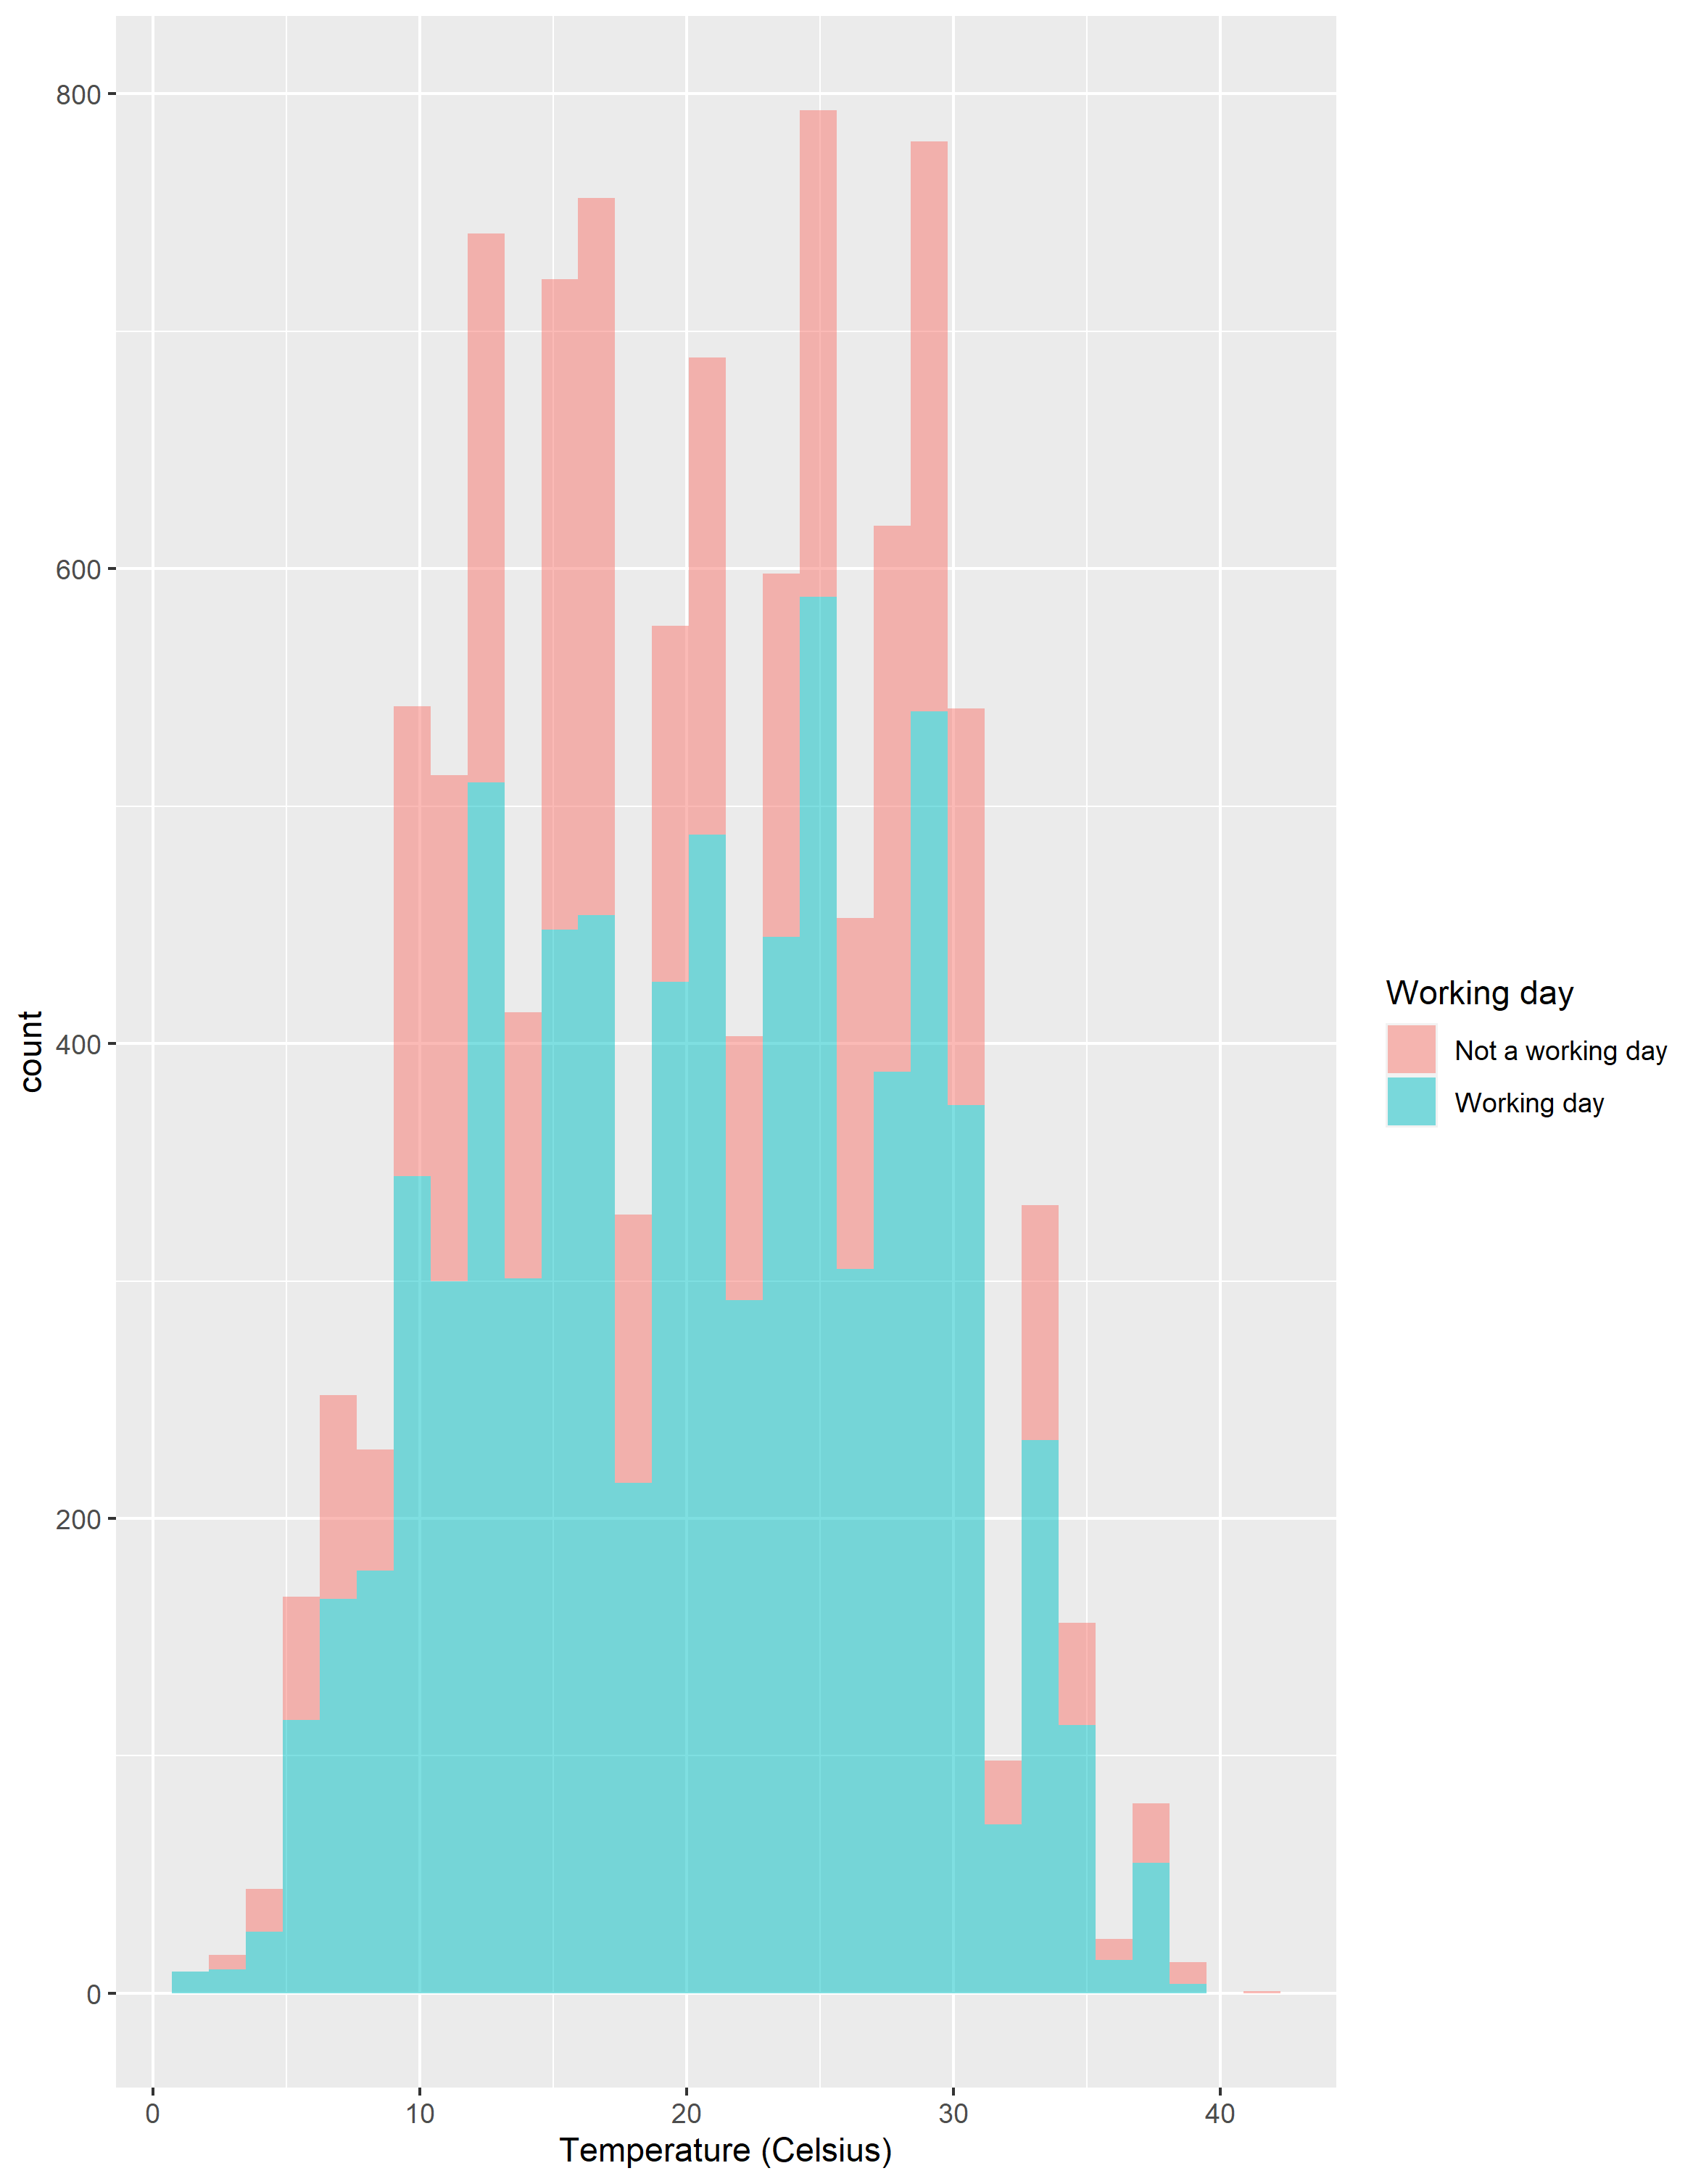
\includegraphics[scale = 0.3]{Figures/hist_temp_workingday.png}
    \caption{Temperature vs Count (by working day)}
    \label{fig:my_label}
\end{figure}
Not surprisingly, when people aren't working, the bike counts are higher. Moreover, warmer temperatures tend to evoke more people to bike, regardless of work day.

\begin{figure}[htp]
    \centering
    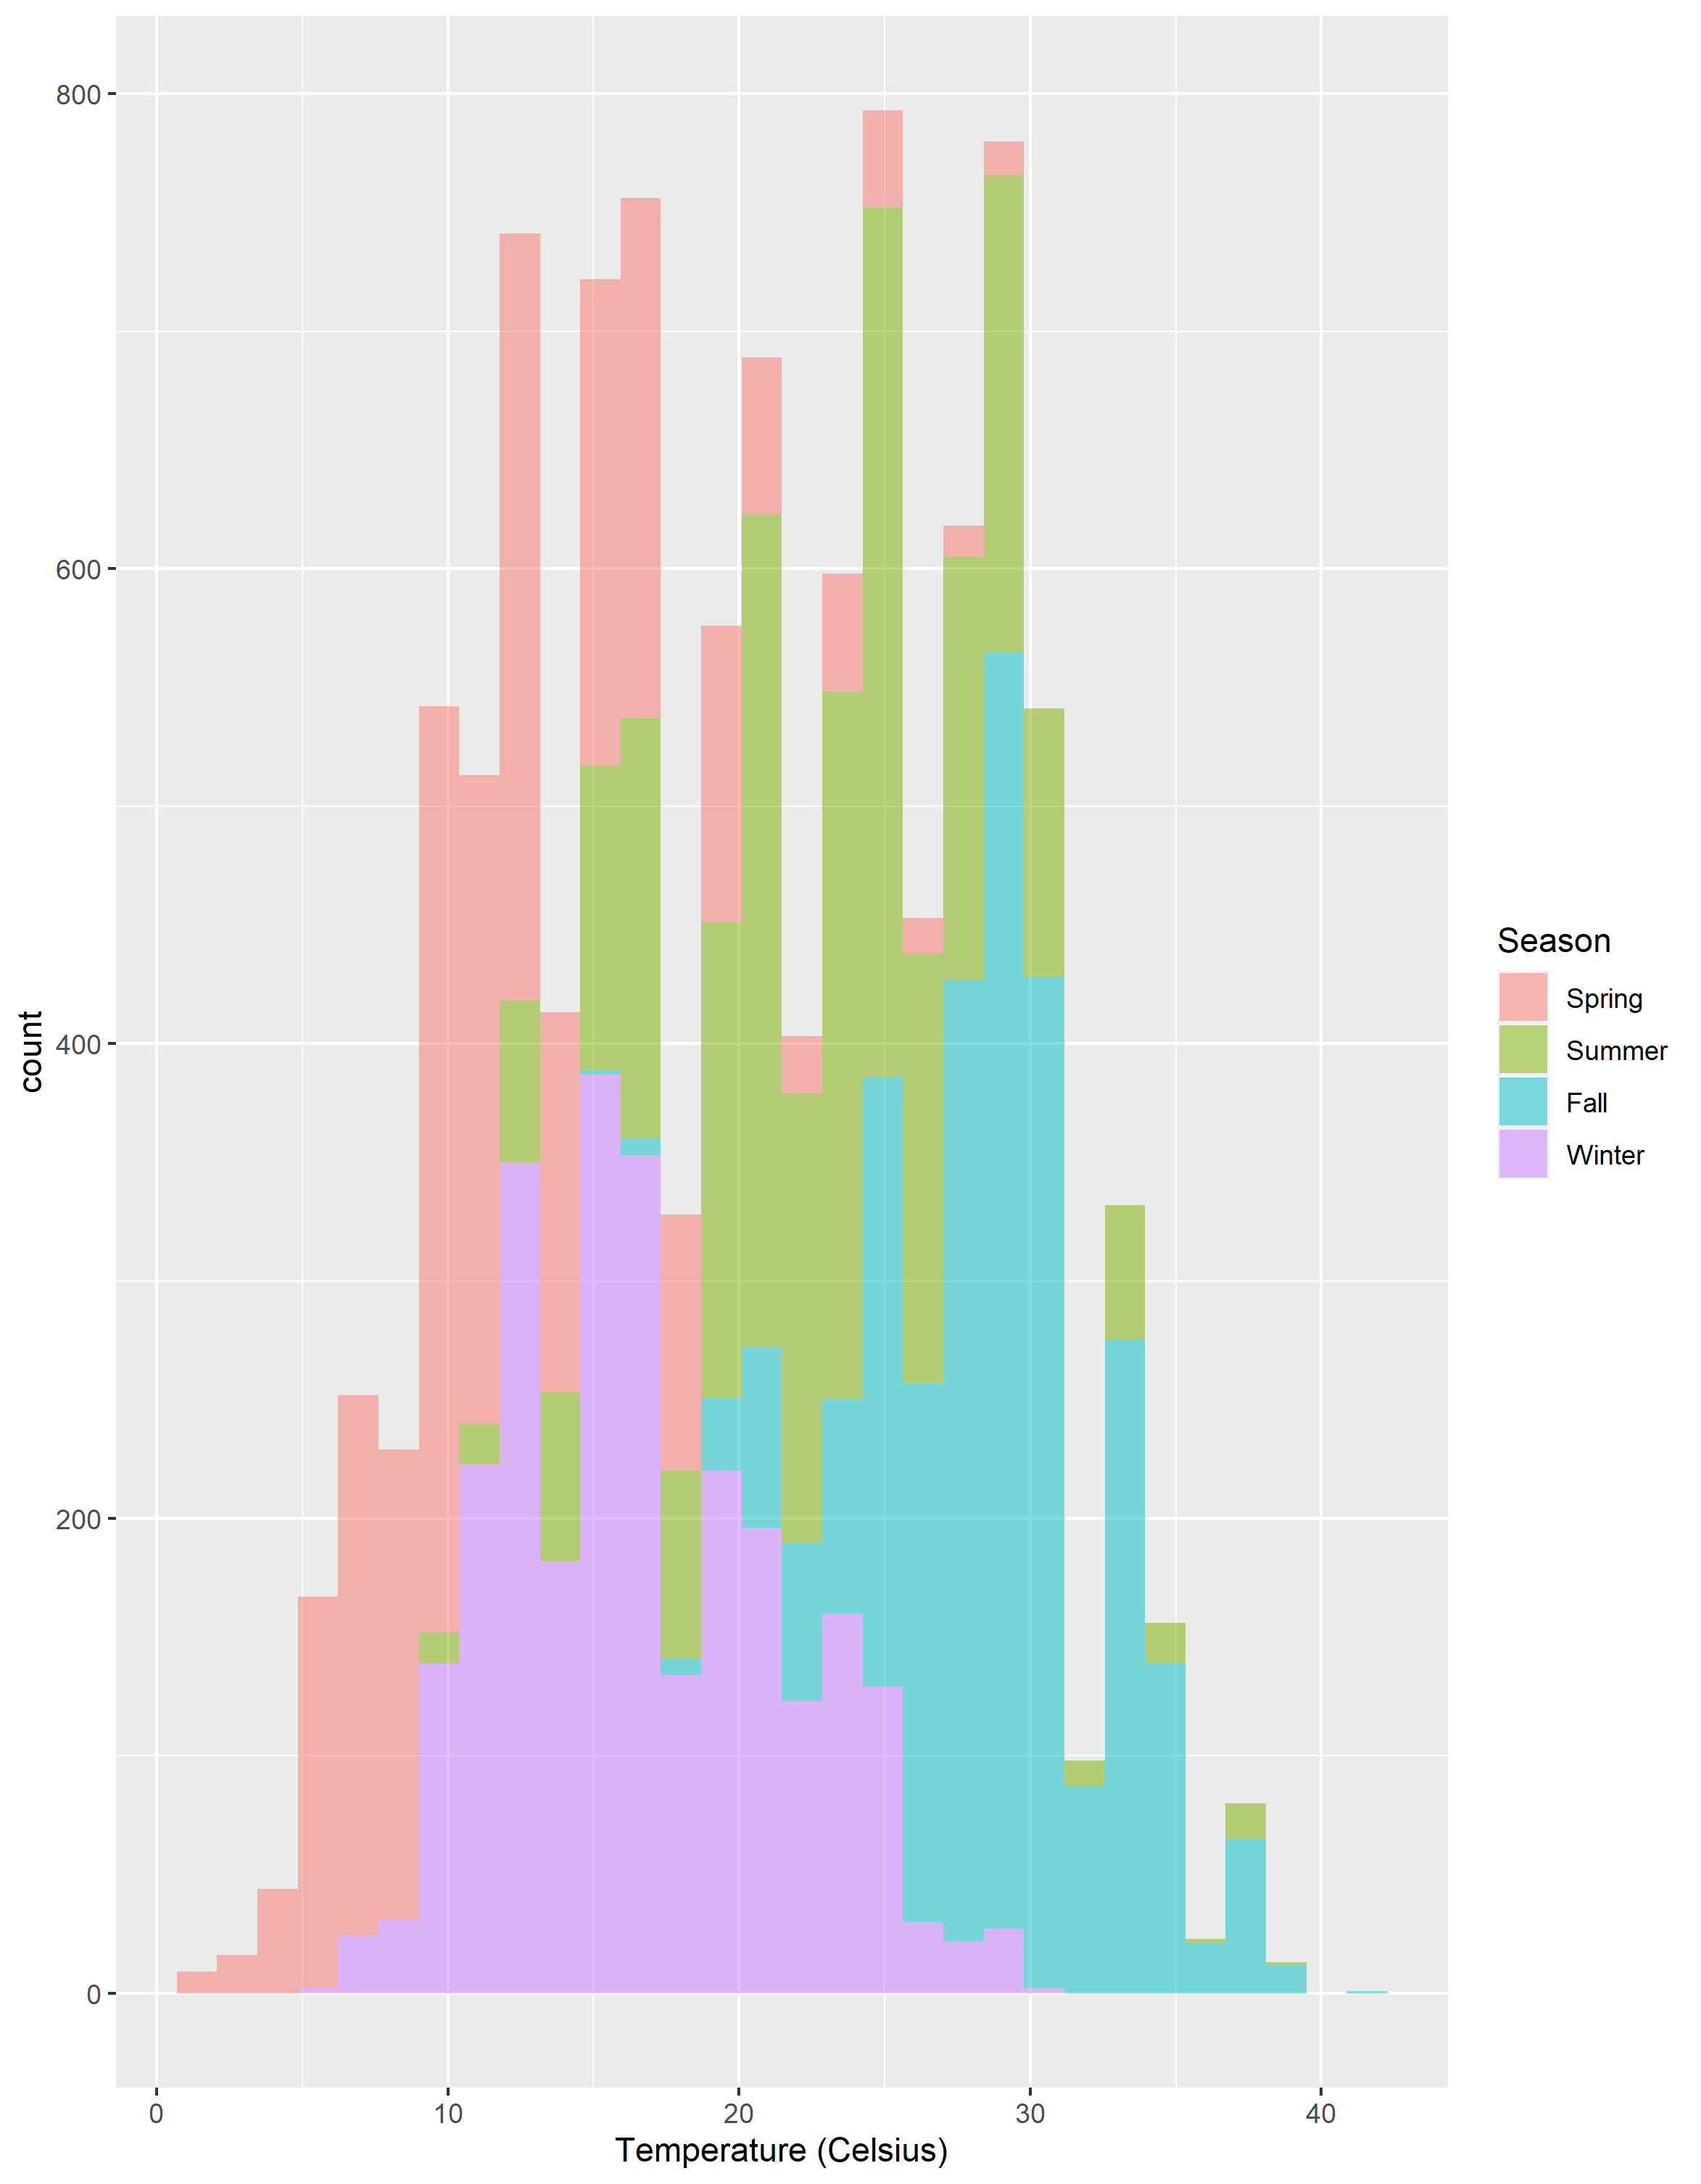
\includegraphics[scale = 0.3]{Figures/hist_temp_season.png}
    \caption{Temperature vs Count (by  season)}
    \label{fig:my_label}
\end{figure}
Similarly, we see here that warmer temperatures produce more bike counts: summer and spring evidently have higher bikes counts than winter and fall. \\
\indent Another feature that caught my eye was 'atemp', or the temperature that it feels like, since this feels like a redundant feature since we already have temperature. Let's take a look at a correlation matrix of the covariates.

\begin{figure}[htp]
    \centering
    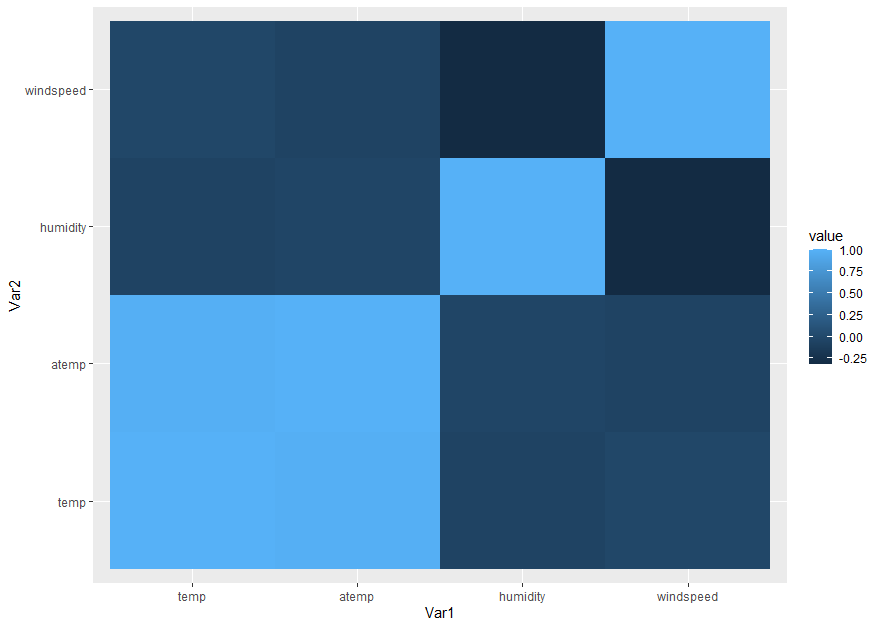
\includegraphics[scale = 0.25]{Figures/correlation_matrix.png}
    \caption{Correlation matrix}
    \label{fig:my_label}
\end{figure}
As expected, atemp and temp are highly correlated. This might be useful information when we attempt to build a model.

\section{Model}
The first thing we do is construct a simple multiple regression model. 
$$\mathbb{E}(\text{Bike Count}) = \beta_{0} + \beta_{1} \cdot \text{temp} + \beta_{2} \cdot \text{humidity} + \beta_{3} \cdot \text{windspeed} + \beta_4 \cdot \text{workingday}
$$
From this model, we find that the humidity and temperature are highly significant (p-value $<2e$-$16)$. Next, we look test for interaction.
$$\mathbb{E}(\text{Bike Count}) = \beta_{0} + \beta_{1} \cdot \text{temp} + \beta_{2} \cdot \text{humidity} + \beta_{3} \cdot \text{windspeed}+ $$$$ \beta_4 \cdot \text{workingday} + \beta_5 \cdot \text{temp*humidity}
$$
which is indeed significant. Using an F-test to compare the two models, we also get a significant p-value, indicating that the second model is preferred. Lastly, we include all the variables in the model.
$$\mathbb{E}(\text{Bike Count}) = \beta_{0} + \beta_{1} \cdot \text{temp} + \beta_{2} \cdot \text{humidity} + \beta_{3} \cdot \text{windspeed} +$$$$ \beta_4 \cdot \text{workingday} + \beta_5 \cdot \text{season} + \beta_6 \cdot \text{holiday}
$$
Coefficients for temperature, humidity, windspeed, winter, and fall were significant.\\
\section{PCA}
\indent As was previously mentioned, temp and atemp were highly correlated. This brings up the possibility of first conducting PCA. Since PCA only works with continuous variables, we only include temp, atemp, humidity, and windspeed. In R, I found that the first 3 principal components retained $99\%$ of the variability in the original data. We use these components as our new covariate. \\
\indent Using a training set size of $70\%$ and a test set size of $30\%$, we produced a model with an AUC of 0.64.

\section*{Discussion}
It was an interesting challenge to explore this dataset. I thought it was unique because it had both categorical and continuous data, which forced me to find ways to use different methods such as PCA and linear regression to make use of both of them. In the end, I think the multiple linear regression models worked quite well, as they produced many significant coefficients. I think it would be interesting to try more complicated models such as neural networks or random forests.


\end{document}
